\documentclass[tesis.tex]{subfiles}

\begin{document}
	
\chapter{Grafos de Cayley.} \label{seccion_treewidth}

Las referencias centrales de este capítulo son \cite{diekert2017context}, \cite{kuske2005logical} y \cite{diestel2005graph}.





\section{Treewidth.}

Dado que el grafo de Cayley de todo grupo libre se puede tomar para que sea un árbol es razonable pensar que todo grupo virtualmente libre es tal que su grafo de Cayley se parezca a un árbol. 

Una noción que podemos tomar de la teoría de grafos para modelizar esto es el de tener un treewidth finito.

\begin{deff}\label{desc-arbol}
	Una \emph{descomposición en un árbol} de un grafo $X$ es un árbol $T$ y un mapa 
	\[
	X: V(T) \to {\cal P}(V(\Gamma))
	\]
	Le vamos a pedir que cumpla las siguientes condiciones:
	\begin{enumerate}
		\item[\textbf{T1.}] Para todo vértice $v \in V(\Gamma)$ debe existir $t \in V(T)$ tal que $x \in X(t)$. 
		\item[\textbf{T2.}] Para toda arista $e$ entre dos vértices $v,w \in V(\Gamma)$ debe existir $t \in V(T)$ tal que $v,w \in X(t)$.
		\item[\textbf{T3.}] Si $v \in V(\Gamma)$ es tal que $v \in X(t) \cap X(s)$ luego $v \in X_r$ para todo $r$ en la geodésica que va desde $s$ a $t$ dentro de $T$. En otras palabras esto es que $\{ t \in V(T) :  v \in X(t) \}$ forma un subárbol. 
	\end{enumerate} 
\end{deff}
\smallskip

La idea de la descomposición es que los \emph{bolsones} $X(t) \in {\cal P}(V(T))$ no tengan muchos vértices si es que queremos modelizar que el grafo se parezca a un árbol. Esto nos conduce a la siguiente definición.

\begin{deff}
	El \emph{bagsize} de una descomposición en un árbol $T$ de un grafo $X$ es el siguiente valor:
	\begin{equation*}
		bs(X,T) = \{ \sup |X(t)|, \ t \in V(T) : T \ \text{descomposición de} \ \Gamma \} - 1
	\end{equation*}
	Un grafo $X$ tiene \emph{treewidth finito} si existe una descomposición en un árbol de bagsize finito.	
\end{deff}
\begin{ej}\label{desc-arbol-arbol}
	En particular si el grafo $X$ es un árbol notemos que tiene treewidth exactamente igual a 1.
	
	Una manera de probarlo es tomar $T$ la subdivisión baricéntrica de $X$. 
	Dada una arista $(x,y)$ consideramos el baricentro como la siguiente suma formal
	\[
	b(x,y)  = \frac{x+y}{2}.
	\]
	
	
	Con estas definiciones podemos definir la subdivisión baricéntrica del árbol $X$.
	Va a ser un árbol $T$ tal que tiene como vértices a 
	\[
	V(T) = \{ b(x,y) \ | \ (x,y) \in E(\Gamma) \} \cup \{  x \ | \ x \in V(\Gamma)  \}.
	\]
	Las aristas están formadas por 
	\[
	E(T) = \{  (x,b(x,y)) \ | \ (x,y) \in E(\Gamma) \}.
	\]
	Consideramos la siguiente función $X: V(T) \to {\cal P}(V(\Gamma))$  
	\[
	X(t) = 
	\begin{cases}
		\{ x \} \ & \text{si} \ t = x 				\\
		\{ (x,y)  \} \ &\text{si} \ t = b(x,y).
	\end{cases}
	\]
	
	Por como los definimos es evidente que $|X(t)| \le 2$ para todo $t \in V(T)$.
	De esta manera si vemos que se trata de una descomposición en un árbol tendremos probado que $bs(X,T) = 1$ tal como queríamos ver.
	
	Finalmente veamos que se trata de una descomposición. Corroboremos que cumple las tres condiciones necesarias.
	\begin{enumerate}
		\item[\textbf{T1.}] 
		Sea $x \in V(\Gamma)$ luego consideremos $X(x) = \{ x \}$ dado que $x \in V(T)$ por construcción de la subdivisión baricéntrica.
		
		\item[\textbf{T2.}] 
		Dado $(x,y) \in E(\Gamma)$ consideramos $X({b(x,y)}) = \{ x,y \} $ de manera que tanto $x$ como $y$ están en un mismo bolsón.
		
		\item[\textbf{T3.}] 
		Sea $x \in V(\Gamma)$, queremos ver que $\{ t \in V(T) :  v \in X(t) \}$ resulta ser un subárbol de $T$.		
		Para empezar tenemos que $x \in X(t)$ si y solo sí $t = b(x,y)$ para cierta arista $(x,y) \in E(\Gamma)$ o bien $t = x$.
		De esta manera el subárbol que nos queda es conexo porque tenemos $(x,b(x,y))$ para toda arista $(x,y) \in E(\Gamma)$ y no tiene ciclos porque no hay más aristas entre estos vértices de la subdivisión baricéntrica del árbol $X$.
	\end{enumerate}
\end{ej}

Veamos ahora una propiedad que tienen los caminos en los grafos que tienen una descomposición en un árbol.

\begin{prop}\label{prop-camino-desc}
	Sea $\Gamma$ grafo tal que tiene una descomposición en un árbol $T$.
	Sean $X,Y,Z$ bolsones tales que el vértice correspondiente a $Z$ en el árbol $T$ está en la geodésica que va de $X$ a $Y$. 
	Sean $x \in X, y \in Y$ tales que $x = x_0 \dots x_n=y$ es algún camino en $\Gamma$ conectándolos.
	Entonces debe existir algún $ 0 \le i \le n$ tal que $x_i \in Z$. 
\end{prop}

\begin{proof}	
	Vamos a demostrarlo haciendo inducción en la longitud $n$ del camino. 
	El caso base es que $n = 0$ por lo tanto $x=y$. 
	En este caso por ser una descomposición en un árbol tenemos que usando la tercer propiedad que $x \in Z$ también.
	
	Para el paso inductivo tomemos $X'$ bolsón que contiene tanto a $x$ como a $x_1$ que sabemos existe por ser una de las propiedades de las descomposiciones en árboles.
	Si este bolsón $X'$ es $Z$ ya está porque nos alcanza con tomar $i=1$ de manera que $x_1 \in Z$.
	En el caso que esto no ocurra miramos el camino de longitud $n-1$ dado por $x_1 x_2 \dots x_n = y$ y usando la hipótesis inductiva llegamos al resultado.	
\end{proof}

\begin{prop}\label{prop_tw_finitos_bolsones}
	Sea $\Gamma$ un grafo localmente finito con treewidth finito entonces podemos tomar una descomposición en un árbol de $\Gamma$ de manera que para todo $v \in V(\Gamma)$ valga que:
	\[
	| \{  t \in V(T) : \ v \in X(t)  \} | < \infty.
	\]
\end{prop}
\begin{proof}
	Por la propiedad \textbf{T2} de la descomposición en un árbol tenemos que para cada arista $(u,v) \in E(\Gamma)$ existe un bolsón que denotaremos $X_{(u,v)}$ tal que $u,v \in X_{(u,v)}$.
	Si hacemos esto para cada una de las aristas incidentes a algún vértice $v \in V(\Gamma)$ obtenemos finitos bolsones y así finitos vértices en el árbol $T$.
	Consideremos el subárbol finito que se genera a partir de estos finitos vértices, llamesmolo $T'$.
	Lo que hacemos es sacar a $v$ de los bolsones que correspondan a vértices que no estén en $T'$.
	Esto es que nuestra nueva descomposición en un árbol va a ser $Y: V(T) \to {\cal P}(V(\Gamma))$ dada por 
	
	\[
	Y(t) = 
	\begin{cases}
		X(t)  \ \  \text{si} \ \  t \in T' \\
		X(t) \setminus \{  v \} \ \  \text{si} \ \  t \in T'
	\end{cases}
	\]
	haciendo esto mismo para cada uno de los vértices del grafo $\Gamma$.
	
	Finalmente chequeamos que sea trata de una descomposición en un árbol.
	Las primeras dos condiciones \textbf{T1} y \textbf{T2} se siguen cumpliendo.
	La condición \textbf{T3} es válida también porque justamente dejamos que todo $v$ esté en un bolsón $ X(t)$ con $t \in T'$ un subárbol, por lo tanto toda geodésica que tomemos va a estar en este subárbol.
	Dado que $X$ ya era una descomposición tenemos que $v \in X(s)$ para todo $s$ en toda geodésica.
	Esta descomposición sigue siendo finita porque todo bolsón a lo sumo mantiene su orden.	
\end{proof}

\begin{deff}
	Sea $\Gamma$ un grafo y $C \subseteq V(\Gamma)$ un conjunto de vértices entonces definimos los \emph{vecinos de $C$} por medio de 
	\[
	N(C) = \{ v \in V(\Gamma) : \exists w \in C, \ vw \in E(\Gamma) \}.
	\]
	De esta manera podemos definir recursivamente los l-ésimos vecinos por medio de $N^l(C) = N(N^{l-1}(C))$.
\end{deff}

\begin{obs}
	Esta definición la podemos escribir de manera más concisa como $N^l (C) = \{ v \in V(\Gamma) : \ \exists w \in C, \  d(v,w) \le l  \}$.
\end{obs}

\begin{prop}\label{prop-vecinos-desc}
	Si $(X(t))_{t \in V(T)}$ es una descomposición en un árbol $T$ para un grafo $\Gamma$ entonces si tomamos como bolsones a $N^l(X(t))$ también tenemos una descomposición en un árbol.
\end{prop}
\begin{proof}
	Equivalentemente queremos ver que el mapa $Y: V(T) \to {\cal P}(V(\Gamma))$ dado por $Y(t) = N^l(X(t))$ nos da otra descomposición en un árbol del grafo $\Gamma$.
	
	Probemos este resultado haciendo inducción en $l$.
	
	Consideremos el caso base $l=1$.
	En este caso, las dos primeras condiciones de la descomposición en un árbol \textbf{T1} y \textbf{T2} se siguen cumpliendo porque no hicimos más que agrandar los bolsones. 
	Esto es que si $X(t)$ era un bolsón luego $X(t) \subseteq Y(t)$.
	
	Debemos ver que cumple \textbf{T3}.
	Partamos de un vértice $x \in V(\Gamma)$ tal que $x \in Y(s) \cap Y(t)$ y veamos que si $r \in V(T)$ está en la geodésica de $t$ a $s$ entonces $x \in Y(r)$.
	Notemos que en este caso debe existir algún $y \in Y_s$ tal que $(x,y) \in E(\Gamma)$.
	Análogamente existe $z \in Y(t)$ tal que $(x,z) \in E(\Gamma)$.
	Si no fuera así tendríamos que $x \in X(s) \cap X(t)$ y esta condición ya se cumpliría por ser los bolsones de una descomposición.
	Entonces si usamos la proposición \ref{prop-camino-desc} tomando el camino $yxz$ tenemos que alguno de estos tres vértices debe estar en $X_r$.
	De esta manera $x \in Y(r)$ tal como queríamos ver.
	
	El paso inductivo se sigue directamente del caso base porque si sabemos que $N^{l-1}(X(t))$ forma una descomposición de un árbol usamos el caso base para ver que los vecinos de esta descomposición lo siguen siendo y con esto terminamos de probarlo porque $N^l(X(t)) = N (N^{l-1})(X(t))$.
\end{proof}
\medskip

\begin{deff}
	Dado un grafo $X$ y un conjunto de vértices $C \subseteq V(\Gamma)$ definimos el \emph{borde de vértices} de $C$ como:
	\[
	\beta C =  N(C) \cap N(\ol{ C})
	\] 
	por otro lado tenemos que el \emph{borde de aristas} de $C \subseteq V(\Gamma)$ se define como:	
	\[
	\delta C = \{  (x,y) | x \in C, y \in \ol C    \}.
	\]
\end{deff}

\todo[inline]{Escribir con la notación más estándar que aparece en el paper de Krön y factorizar la construcción.}

\begin{center}
	\missingfigure[figwidth=6cm]{Dibujo ilustrativo.}
\end{center}

\begin{ej}\label{desc-grafo-cayley}%[Descomposición válida para todo grupo finitamente generado].
	
	Construyamos una descomposición en un árbol que podemos hacer en general para todos los grafos de Cayley de grupos finitamente generados. 
	Consideremos el grafo $\Gamma = \text{Cay}(G,A)$ para cierto conjunto de generadores $A$ finito.
	
	
	Sea $V_n = \Gamma \setminus B_n(1) $ tal que $V_0 = \Gamma \setminus \{1\}$. 
	Los vértices del árbol $T$ van a estar dados por los siguientes conjuntos,
	\[
	V(T) = \{  \beta C : C \subseteq V_n \ \text{componente conexa}   \} \cup \{ 1 \}
	\]
	esto es todas las bordes de vértices de las componentes conexas que nos quedan cuando consideramos algún $V_n$. 
	Las aristas entonces van a estar dadas por lo siguiente,
	\[
	E(T) = \{ (\beta C , \beta D) : C \subseteq D \subseteq V_n, \ C \subset V_{n+1}   \} \cup \{  (1, \beta C) : C \subseteq V_0  \}
	\]
	esto es que $C$ es una componente conexa del grafo que queda de sacarla la bola de radio un número mayor que el que está $D$.
	Notemos en particular que por como definimos este grafo $T$ resulta que si $C$ es una componente conexa de $V_n$ entonces solo existe una única arista $(\beta C, \beta D)$ tal que $D \subseteq V_{n-1}$. 
	Esto se debe a que al ser $C$ conexo entonces como $V_{n-1} \subseteq V_{n}$ en particular $C \subseteq V_{n}$ y debe estar contenida en una sola componente conexa $D \subseteq V_{n-1}.$
	
	
	Podemos ver que así como lo construimos tenemos que el grafo $T$ resulta ser un árbol tal que su raíz es $1$. 
	
	Para ver que es un árbol veamos primero que es conexo. Dado un vértice $\beta C \in V(T)$ vamos a armar un camino que lo conecte con la raíz del árbol $1$. 
	Usemos inducción en el $n$ tal que $C$ es una componente conexa de $V_n$. 
	El caso base es algún $C$ tal que es una componente conexa de $V_1$ y queremos armarnos un camino que lo una con $B_1(\Gamma)$. 
	Por construcción de las aristas necesariamente tenemos que $(1, \beta C) \in E(T)$.
		
	Para el paso inductivo supongamos para cualquier borde de una componente conexa de $V_{n-1}$ tenemos un camino que lo une con la raíz $1$ y veamos de construirnos un camino con cualquier borde de una componente conexa $C \subseteq V_n$.
	De esta manera debe existir $D$ componente conexa de $V_{n-1}$ tal que $C \subseteq D$. Esto es porque $V_{n-1} \subseteq V_{n}$ y al ser $C$ un conexo si interseca alguna de las componentes conexas de $V_{n-1}$ debe estar contenida en ella. 
	Necesariamente debe intersecar a alguna de estas componentes conexas porque particionan al espacio.
	Así vimos que existe una arista $(\beta C, \beta D)$ y ahora usando la hipótesis inductiva obtenemos un camino de $1$ a $\beta C$.
	Concluimos que el grafo $T$ es conexo.   
	
	% Otra manera que se me ocurrió es tomar un ciclo de longitud mínimo y llegar a un absurdo achicandolo. Creo que es más corto pero no me convence.
	Para terminar de ver que es un árbol veamos que es acíclico. 
	Dado un camino cerrado $\sigma$ en $T$ probemos que necesariamente tiene que repetirse algún vértice por lo tanto ningún camino cerrado puede ser un ciclo. Vamos a probarlo usando inducción en el máximo $n \in \NN$ tal que $C \in V_n$ y $\beta C$ es uno de los vértices en el camino. 
	%Notemos que está bien definido porque los caminos cerrados son compactos.
	Para el caso base notemos que si $\sigma$ es un camino cerrado tal que el máximo $n$ que aparece es $n=1$ entonces necesariamente $\sigma$ es idéntico al camino constante fijo en $1$.
	%reescribir esto!
	Para el paso inductivo supongamos que para todo camino cerrado con máximo $m \in \NN$ tal que algún vértice que aparece en este camino es una componente conexa de $V_m$ resulta ser $n-1$ entonces este camino no es un ciclo. Veamos que si $m=n$ entonces este camino cerrado también resulta ser un ciclo.
	
	Partamos de un camino tal que pasa por $\beta C$ con $C \subseteq V_n$. 
	Como no existe $(\beta C, \beta C') \in E(T)$ tal que $C,C'$ sean componentes conexas de un mismo $V_n$ por la definición que dimos de las aristas necesariamente tiene que haber una arista con alguna componente conexa $D \in V_{n-1}$ dado que $n$ es máximo en este camino cerrado.   
	Como vimos anteriormente solamente hay una única arista que una a $\beta C$ con alguna $\beta D$ con $D \subseteq V_{n-1}$. 
	Esto nos dice que si el camino cerrado pasa por la arista $(\beta C, \beta D)$ necesariamente debe volver a pasar por la arista $(\beta C, \beta D)$ por lo tanto no es un ciclo. 
	Concluimos que el grafo $T$ es acíclico y por lo tanto como es conexo también resulta que $T$ es un árbol.
	
	Para ver que es una descomposición de árboles debemos ver que cumple las tres condiciones \ref{desc-arbol} de la definición. 
	\begin{enumerate}
		\item[\textbf{T1.}] La primera condición la cumple por como lo definimos porque cualquier vértice del grafo $g \in V(\Gamma)$ 
		es tal que existe $n \in \NN$ de manera que $d(1,g)=n$, por lo que está en alguna componente conexa $C \subseteq V_{n-1}$. 
		En particular como la distancia es exactamente $n$ tiene que existir una arista $(g,g') \in E(\Gamma)$ con un vértice $g' \in V_{n-1}$ y por lo tanto $g \in \beta C$.
		
		\item[\textbf{T2.}] La segunda condición partimos de una arista $(g,h) \in E(\Gamma)$ luego miramos las distancias que hay al $1$ de ambos vértices para conseguirnos el bolsón adecuado. 
		Supongamos que ambas están a la misma distancia del $1$. En tal caso sea $n$ tal que 
		\[
			d(g,1)=n = d(h,1)
		\] 
		luego si miramos $V_{n-1}$ notemos que tienen que estar en la misma componente conexa porque existe una arista entre ambos vértices. Sea esta componente $C$ luego como están a distancia exactamente $n$ ambas están en el borde, esto es que $g,h \in \beta C$ tal como queríamos ver. 
		El otro caso es que 
		\[
			d(g,1)=n < n+1 = d(h,1)
		\] 
		y en este caso como están conectadas resulta que están en $\beta C$ si $C$ es la componente conexa que contiene a $h$ en $V_n$ por definición del borde de un conjunto de vértices de un grafo.
		
		\item[\textbf{T3.}] Para la tercera condición supongamos que hay $g \in V(\Gamma)$ tal que está en la intersección de dos bolsones $\beta C \cap \beta D$. 
		Queremos ver que está en todos los bolsones que aparecen en la geodésica de $\beta C$ a $\beta D$ en el árbol T. 
		Si $d(g,1) = n$ luego solo puede estar en la frontera de alguna componente conexa $C$ tal que esté en $V_{i}$ para $i\in \{n-1, n, n+1\}$. 
		Supongamos que $D \subseteq V_{n}$, en tal caso vale que $D \nsubseteq V_{n}$ porque sino tendríamos que resulta ser la misma componente conexa. 
		Sin pérdida de generalidad supongamos que $C \subset V_n$ mientras que $D \subset V_{n+1}$. 
		Como ambas son componentes conexas luego si hay una intersección tiene que haber una contención, esto es que $D \subseteq C$. 
		De esta manera vemos que $(\beta C, \beta D) \in E(T)$ por lo tanto como están unidos por una arista la geodésica es justamente esta arista.
		
	\end{enumerate}
\end{ej}

\section{Cuasisometrías.}

Nuestro objetivo es introducir las cuasisometrías para garantizar que la propiedad de tener treewidth finito no dependa de los generadores elegidos.
Esta subsección sigue los textos de \cite{bridson2013metric} y de \cite{loh2017geometric}.

\begin{deff}
	Sean $(X,d_X),(Y,d_Y)$ espacios métricos. 
	Una \emph{cuasisometría} es una función $f:X \to Y$ tal que:
	\begin{itemize}
		\item[\textbf{Q1.}] Existe constante $A > 0$ tal que para todo par de puntos $x_1,x_2 \in X$ hace valer la siguientes desigualdades
		\[
		\frac{1}{A} d_X(x_1,x_2) - A \le d_Y(f(x_1),f(x_2)) \le A d_X(x_1,x_2) + A
		\]
		\item[\textbf{Q2.}] Existe una constante $C \ge 0$ tal que para todo punto $y \in Y$ debe existir $x \in X$ de manera que 
		\[
		d(y,f(x)) \le C
		\]
	\end{itemize}
\end{deff}

Intuitivamente una cuasisometría entre espacios métricos nos dice que estos resultan ser bastante similares al menos desde cierta distancia. 
\medskip
\begin{prop}
	Si existe $f:X \to Y$ cuasisometría entonces también debe existir $g:Y \to X$ cuasisometría y constantes positivas $C,D \in \RR$ tal que:
	\begin{itemize}
		\item $d(g \circ f (x), x) < C$ para todo $x \in X$.
		\item $d(f \circ g (y), y) < D$ para todo $y \in Y$. 
	\end{itemize}
\end{prop}
\begin{proof}
	Ver \cite{loh2017geometric}.
\end{proof}

\begin{deff}
	Dos espacios métricos que se dicen \emph{cuasisométricos} si existe una cuasisometría entre ellos.
\end{deff}

Vale el siguiente resultado.
\begin{prop}
	Ser cuasisométricos es una relación de equivalencia entre espacios métricos.
\end{prop}
\begin{proof}
	Ver \cite{loh2017geometric}.
\end{proof}


Todo grafo de Cayley lo podemos pensar como un espacio métrico tal como lo definimos en la sección \ref{seccion_treewidth}.  
Veamos que esto no depende de los generadores que hayamos elegido.

\begin{prop}
	Sea $G$ grupo \fg por $\Sigma$ y $\Delta$ conjuntos finitos entonces $\text{Cay}(G,\Sigma)$ y $\text{Cay}(G, \Delta)$ son cuasisométricos entre sí.
\end{prop}

\begin{proof}
	Resultado estándar. Ver \cite{bridson2013metric}.
\end{proof}


%\begin{obs}
%	Si nos restringimos a que los espacios métricos sean grafos podemos redefinir una cuasisometría para que sea una función de los vértices de un grafo a los del otro.
%	Esto es si tenemos dos grafos $\Gamma_1$ y $\Gamma_2$ entonces son cuasisométricos como espacios métricos si y solo si existe $f:V(\Gamma_1) \to V(\Gamma_2)$ tal que 
%	\begin{itemize}
%		\item Para todo $v,w \in V(\Gamma_1)$ existe constante $A > 0$ tal que 
%		\[
%		\frac{1}{A} d_X(v,w) - A \le d_Y(f(v),f(w)) \le A d_X(v,w) + A
%		\]
%		\item Existe una constante real $C \ge 0$ tal que para todo vértice $y \in V(\Gamma_2)$ existe $v \in V(\Gamma_1)$ tal que 
%		\[
%		d(y,f(v)) \le C
%		\]
%	\end{itemize}
%	
%	Para esto si tenemos una cuasisometría $g$ como espacios métrices definamos una sobre los vértices $f$ de la siguiente manera.
%	Por cada vértice $v \in V(\Gamma_1)$ consideremos $g(v) \in \Gamma_2$. 
%	Si $g(v) \in V(\Gamma_2)$ tomamos $f(v)=g(v)$.
%	El otro caso es que $g(v)$ cae en el medio de alguna arista $xy \in E(\Gamma_2)$. 
%	Supongamos que $d(g(v),x) \le \frac{1}{2}$ porque la distancia máxima con alguno de los vértices debe ser no más de $\frac{1}{2}$ porque justamente las aristas son isométricas con el intervalo $[0,1]$. 
%	En este caso definamos $f(v) = x$.
%	Notemos ahora que la distancia entre dos vértices por medio de $f$ a lo sumo aumenta. 
%	Tenemos que 
%	\[
%	d(f(v),f(w) \le d (g(v),g(w)) + 1
%	\]
%	para $v,w \in V(\Gamma_1)$ porque a lo sumo las imágenes por $g$ están a distancia $\frac{1}{2}$ de alguno de los vértices.
%	De esta manera notemos que si tomamos la constante $C+1$ nos sirve.
%	Para ver que la imagen es cuasidensa idénticamente tomando $C+1$ nos sirve.
%	En definitiva $f$ definida de esta manera es una cuasisometría con constante $C+1$.	
%\end{obs}

Veamos ahora que el treewidth es un invariante por cuasisometría y entonces no depende de los generadores elegidos y por lo tanto es una propiedad intrínseca del grupo. 

\begin{prop} \label{treewidth-inv}
	El treewidth finito es un invariante por cuasisometría para grafos con grado acotado uniformemente.
\end{prop}

\begin{proof}
	Si tenemos una cuasisometría $f:\Gamma_1 \to \Gamma_2$ tal que $\Gamma_2$ tiene treewidth finito $k \in \NN$, nos gustaría ver que $\Gamma_1$ también tiene esta propiedad.
	Consideremos $l$ tal que $d(f(v),f(w)) \le l$ para vértices $v,w \in V(\Gamma_1)$ que estén conectados por una arista.
	Esto lo podemos tomar porque al ser una cuasisometría 
	\[
	d(f(v),f(w)) \le C d(v,w) + C  \le 2C
	\]
	entonces basta con tomar $l \ge C+1$.
	
	Veamos de armarnos la descomposición en un árbol $T$ para $\Gamma_1$.	
	Tomaremos como árbol para descomposición al mismo $T$ que usamos para $\Gamma_2$.
	Sean $X(t)$ los bolsones de esta descomposición. 
	Recordemos que por \ref{prop-vecinos-desc} si tomamos $N^l(X(t))$ los vecinos del bolsón $X(t)$ que están a distancia no mayor a $l$ seguimos teniendo una descomposición.  
	Consideraremos los bolsones $Y(t) = f^{-1}(N^l(X(t)))$ de vértices en $\Gamma_1$. 
	
	Debemos ver que cumplen las tres propiedades.
	
	\begin{enumerate}
		\item[\textbf{T1.}] La primera se cumple puesto que los bolsones $X(t)$ cubren $V(\Gamma_2)$. 
		De esta manera $\bigcup_{t \in T} N^l(X(t)) = V(\Gamma_2)$ y por lo tanto tomando preimagen tenemos que
		\[
		\bigcup_{t \in V(T)} f^{-1} (N^l (X(t))) = \bigcup_{t \in V(T)} Y(t) = f^{-1} (V(\Gamma_2)) = V(\Gamma_1)
		\] 
		donde usamos que la preimagen de la unión es la unión de las preimágenes.
		\item[\textbf{T2.}] La segunda condición usamos que si hay una arista $xy \in E(\Gamma_2)$ luego debe ser que $d(f(x),f(y)) \le l$ por como tomamos a $l$.
		De esta manera como $f(x) \in X(t)$ para algún $t \in V(T)$, notemos que $f(y) \in N^l(X(t))$ también. 
		Tomando preimagen tenemos que $x,y \in f^{-1}(N^l(X(t)))$ y esto es que justamente $x,y \in Y(t)$ para un mismo $t \in V(T)$ tal como queríamos ver.		
		\item[\textbf{T3.}] Para la tercera condición si $x \in Y(t) \cap Y(s)$ queremos ver que $x \in Y(r)$ para todo $r \in V(T)$ que aparezca en la geodésica de $s$ a $t$.
		Como la preimagen de una intersección es lo mismo que la intersección de las preimágenes entonces 
		\[
		x \in f^{-1}(N^l(X(t))) \cap f^{-1}(N^l(X(s))) = f^{-1}(N^l(X(t)) \cap N^l (X(s))
		\]
		de esta manera debe existir $v \in V(\Gamma_2)$ tal que $v \in N^l(X(s)) \cap N^l(X(t))$.
		Ahora usamos que esta es una descomposición sobre $\Gamma_2$ para notar que $v \in N^l(X_r)$.
		Tomando preimagen tenemos que $x \in Y(r)$ tal como queríamos ver.
	\end{enumerate}
	
	Finalmente debemos ver que el tamaño de los bolsones está acotado uniformemente.
	Esto es que exista $k \in \NN$ tal que $|Y(t)| \le k$ para todo $t \in V(T)$.
	Como $\Gamma_2$ tiene treewidth finito tenemos que $|X(t)| \le M$ uniformemente para todo $y \in V(T)$ para cierta $M$. 
	Como el grado de los grafos está acotado uniformemente por alguna constante $d$ tenemos que 
	\[
	|N^l(X(t))| \le d^l |X(t)| \le d^l M.
	\]
	Finalmente notemos que al ser $f$ una cuasisometría tenemos que $|f^{-1}(v)| \le k$ para todo $v \in V(\Gamma_2)$.
	Esto lo podemos ver porque si $f(x) = v = f(y)$ entonces
	\[
	\frac{1}{C}d(x,y) - C \le d( f(x), f(y) ) = 0 \implies d(x,y) \le C^2 < \infty
	\]
	y esta cota es uniforme para todo $v \in \Gamma_2$. 
	Así vemos que,
	\[
	|Y(t)| = |f^{-1}(N^l(X(t)))| \le C^2 d^l M < \infty
	\]
	y tomamos $k$ suficientemente grande para que haga valer esto.
	Concluímos así que la descomposición que nos armamos para $\Gamma_1$ tiene treewidth finito.
\end{proof}

A partir de este resultado podemos ver que la otra manera que teníamos de pensar a los grafos que se parecen a árboles resulta ser más débil. 
El siguiente resultado lo demostramos en el caso general de un grafo tal que los grados de sus vértices están acotados uniformemente. 
Como caso particular tenemos los grafos de Cayley de grupos finitamente generados.


\begin{prop} 
	Un grafo $X$ de grado acotado uniformemente cuasisométrico con un árbol tiene treewidth finito.
\end{prop}
\begin{proof}	
	El grafo $X$ es cuasisométrico a un árbol $T$ y todo árbol por la observación \ref{desc-arbol-arbol} tiene treewidth exactamente $1$.
	Por la proposición anterior \ref{treewidth-inv} como tener treewidth finito es un invariante por cuasisometría vemos que $X$ debe tener treewidth finito tal como queríamos ver.
\end{proof}

\section{Grupos \ic tienen treewidth finito.}

En esta sección probaremos un resultado que fue originalmente probado por Muller--Schupp en \cite{muller1985theory}.
En ese trabajo usan una definición equivalente al treewidth que es que su grafo de Cayley sea $k$-triangulable que resulta ser un poco más técnica.
La demostración que presentamos sigue la exposición del trabajo \cite{diekert2017context}.
Primero una observación sobre el lenguaje del problema de la palabra de un grupo independiente de contexto.

\begin{obs}\label{palabras-wp}
	\todo[]{Tiene que ser un lema.}
	Si tenemos un grupo $G$ tal que es independiente de contexto consideremos $\cal G$ gramática que genera al lenguaje del problema de la palabra, $\WP = L(\cal G)$.
	Si $A$ es una de las variables de esta gramática podemos obtener el lenguaje $L_A$ de palabras generadas a partir de esta variable, donde
	\[
	L_A = \{ w \in \Sigma^*  \ | \ A \deriva w  \}.
	\]
	Veamos que si $v,v' \in L_A$ entonces $v =_G v'$, es decir son el mismo elemento vistos en el grupo $G$. 
	Para eso si tenemos una derivación que en algún momento llega a $S \deriva \beta A \gamma \deriva uvw$ también tenemos otra derivación que deriva en $S \deriva \beta A \gamma  \deriva uv'w$. 
	Es decir que $uvw, u'v'w' \in \WP$ por lo tanto 
	\begin{equation*}
		uvw =_G 1 =_G uv'w \implies v =_G v'
	\end{equation*}
	tal como queríamos ver.
\end{obs}



\todo[]{Completar con historia del resultado.}
El siguiente resultado(...)

\begin{teo} \cite{muller1985theory}
	Todo grupo independiente de contexto es tal que su grafo de Cayley tiene treewidth finito.
\end{teo}
\begin{proof}
	La descomposición que hicimos en \ref{desc-grafo-cayley} es válida para todo grafo de Cayley. 
	Veamos que esta descomposición para un grupo independiente de contexto tiene treewidth finito. 
	Buscamos $k \in \NN$ tal que nos permita acotar $|\beta C| \le k$ para todo $\beta C \in V(T)$. 
	Alcanza con ver que los diámetros de los bolsones $\beta C$ están acotados uniformemente, 
	\todo[]{Factorizar esto en lemita.}
	 esto es que exista $M \in \NN$ tal que 
	\[
	\text{diam}(\beta C) =  \sup_{g,h \in \beta C} d(g,h) \le M
	\] 
	para todo $\beta C$ de la descomposición de árboles.
	Si esto sucede, al ser el grupo finitamente generado por $\Sigma$ entonces $|\beta C| \le |\Sigma|^{M} < \infty$.
	
	
	Dado que $G$ es un grupo independiente de contexto entonces el lenguaje del problema de la palabra para estos generadores $\WP$ tiene una gramática $\cal G$ independiente de contexto que lo genera. 
	Consideremos que está en la forma normal de Chomsky.
	
	Para cada variable $A$ de nuestra gramática podemos considerar el siguiente lenguaje
	\[
	L_A = \{ w \in \Sigma^* : A \deriva w  \}.
	\]
	Para este lenguaje introduzcamos un número natural $k_A \in \NN$ definido por $k_A = \min_{w \in L_A} |w|$. 
	Como tenemos finitas variables en nuestra gramática $\cal G$ podemos considerar $k = \max_{A \in V} k_A$. 
	Veamos que $\text{diam}(\beta C) \le 3k$ para todo $\beta C \in V(T)$.
	
	Sean $g,h \in \beta C$ para cierta $C$ componente conexa de $V_n$, acotemos $d(g,h)$. 
	Para eso consideremos una geodésica $\alpha$ que una $1$ con $g$ y análogamente otra $\gamma$ que una $1$ con $h$. 
	Como $C \cup \beta C$ es conexo podemos tomar un arco $\tau$ que una $g$ con  $h$ dentro de $C \cup \beta C$. 
	De esta manera tenemos un triángulo tal que si leemos las letras que están en la etiqueta del arco empezando desde $1$ y moviéndonos por $\alpha$ leemos la etiqueta $u$. 
	Cuando nos movemos por $\tau$ leemos la etiqueta $v$. Consideremos que esta etiqueta $v$ es tal que $|v|>1$ caso contrario ya tenemos la cota probada. Finalmente leemos la etiqueta $w$ cuando regresamos al $1$ por medio de $\gamma$.
	Como $uvw$ está en un ciclo en el grafo de Cayley entonces $uvw \in  \WP$ y por lo tanto tenemos alguna derivación $S \deriva uvw$.
	
	Ya que tenemos esta derivación $S \deriva uvw$ miremos la primer variable que deriva a $v$ como subpalabra. 
	Esto es que para la subpalabra $v$ sabemos que existe alguna variable $A$ tal que $A \deriva v'v''$ donde $v$ es a su vez una subpalabra de $v'v''$. 
	Tomamos la última variable que aparece en la derivación.
	%Esto es que para la subpalabra $v$ sabemos que debe existir alguna variable $A$ tal que $A \deriva u''vw''$ para $u''$ algún posfijo de $u$ y $w''$ algún prefijo de $w$ y aparece último en esta derivación. 
	Ésta debe existir porque en particular $S$ cumple lo pedido de ser una variable que deriva a una palabra que contiene a $v$ como subpalabra.
	
	Como está en la forma normal de Chomsky sabemos que al ser $|v| \ge 2$ entonces tenemos que la derivación tiene la siguiente pinta
	\begin{equation*}
		S \deriva u'Aw' \Rightarrow_{\cal G} u'BC w' \deriva u'v'v''w'
	\end{equation*}
	donde $B,C$ son otras variables. En particular notemos que $A \deriva v'v''$, $B \deriva v'$ y $C \deriva v''$.
	
	
	Si miramos la geodésica $\alpha$ sabemos que cuando leímos $u'$ habremos llegado a un vértice del grafo $x$, y al estar sobre la geodésica misma tenemos la siguiente igualdad,
	%y que si tomamos el camino que leemos la palabra de menor longitud tenemos que habremos llegado al vértice $y$ que corresponde al haber leído $u'v'$.
	\begin{equation*}
		d(x,g) = d(1,g) - d(1,x).
	\end{equation*}
	Análogamente cuando miramos la geodésica $\gamma$ en la instancia que ya leímos $w'$ saliendo desde $h$ llegamos a cierto vértice $z$ y por la misma razón que en el caso anterior obtenemos
	\begin{equation*}
		d(z,h) = d(1,h) - d(1,z).
	\end{equation*}
	Por otro lado si consideramos el vértice $y$ al que llegamos después de leer $u'v'$ que sabemos que está en el arco $\tau$ dado que $v$ es subpalabra de $v'v''$.
	Usando que $y \in \tau \subseteq C \cup \beta C$ tenemos que $d(1,y) \le n+1 = d(1,g)$ por ser $C$ una componente conexa de $V_n$, entonces vale la siguiente desigualdad
	\begin{equation*}
		d(x,g) = d(1,g) - d(1,x) \le d(1,y) - d(1,x) = d(x,y)
	\end{equation*}
	y análogamente tenemos que $d(z,h) \le d(z,y)$.
	
	
	Por la observación \ref{palabras-wp} notemos que si reemplazamos $v'$ por la palabra de menor tamaño del lenguaje $L_B$ seguimos teniendo un ciclo pero de longitud idéntica o más chica. 
	La palabra $v'$ la leemos justamente cuando vamos del vértice $x$ al vértice $y$, así la distancia  $d(x,y)$ está acotada por la mayor de todas las palabras que puedan derivarse de $B$. 
	Idénticamente hacemos esto para las variables $A$ y $C$.
	Por como definimos a $k$ tenemos las siguientes cotas $d(x,y), d(y,z), d(x,z) \le k$.
	%agregar dibujito, creo que es la manera más clara de explicar esto
	
	\begin{figure}[H]
		\centering
		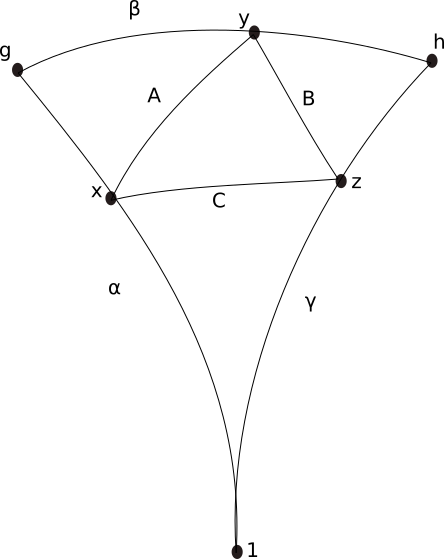
\includegraphics[scale=0.5]{treewidth.png}
		\caption*{}
	\end{figure}
	
	
	
	Ahora estamos listos para ver que $d(g,h) \le 3k$. Usamos la desigualdad triangular tres veces,
	\begin{align*}
		d(g,h) & \le d(g,x) + d(x,z) + d(h,z) \\
		& \le d(x,y) + d(x,z) + d(y,z) \le 3k
	\end{align*}
	tal como queríamos ver.
\end{proof}
	
	
\end{document}